\documentclass{spisok-article}

\usepackage{latexsym,amssymb, amsthm}
\usepackage{subcaption}
\usepackage{physics}
\usepackage{amsmath}
\usepackage{graphicx}
\usepackage{float}
%new calligraphic font for subspaces
\usepackage{euscript}
\newcommand{\cA}{\EuScript{A}}
\newcommand{\cB}{\EuScript{B}}
\newcommand{\cC}{\EuScript{C}}
\newcommand{\cD}{\EuScript{D}}
\newcommand{\cE}{\EuScript{E}}
\newcommand{\cF}{\EuScript{F}}
\newcommand{\cG}{\EuScript{G}}
\newcommand{\cH}{\EuScript{H}}
\newcommand{\cI}{\EuScript{I}}
\newcommand{\cJ}{\EuScript{J}}
\newcommand{\cK}{\EuScript{K}}
\newcommand{\cL}{\EuScript{L}}
\newcommand{\cM}{\EuScript{M}}
\newcommand{\cN}{\EuScript{N}}
\newcommand{\cO}{\EuScript{O}}
\newcommand{\cP}{\EuScript{P}}
\newcommand{\cQ}{\EuScript{Q}}
\newcommand{\cR}{\EuScript{R}}
\newcommand{\cS}{\EuScript{S}}
\newcommand{\cT}{\EuScript{T}}
\newcommand{\cU}{\EuScript{U}}
\newcommand{\cV}{\EuScript{V}}
\newcommand{\cW}{\EuScript{W}}
\newcommand{\cX}{\EuScript{X}}
\newcommand{\cY}{\EuScript{Y}}
\newcommand{\cZ}{\EuScript{Z}}

%font for text indices like transposition X^\mathrm{T}
\newcommand{\rmA}{\mathrm{A}}
\newcommand{\rmB}{\mathrm{B}}
\newcommand{\rmC}{\mathrm{C}}
\newcommand{\rmD}{\mathrm{D}}
\newcommand{\rmE}{\mathrm{E}}
\newcommand{\rmF}{\mathrm{F}}
\newcommand{\rmG}{\mathrm{G}}
\newcommand{\rmH}{\mathrm{H}}
\newcommand{\rmI}{\mathrm{I}}
\newcommand{\rmJ}{\mathrm{J}}
\newcommand{\rmK}{\mathrm{K}}
\newcommand{\rmL}{\mathrm{L}}
\newcommand{\rmM}{\mathrm{M}}
\newcommand{\rmN}{\mathrm{N}}
\newcommand{\rmO}{\mathrm{O}}
\newcommand{\rmP}{\mathrm{P}}
\newcommand{\rmQ}{\mathrm{Q}}
\newcommand{\rmR}{\mathrm{R}}
\newcommand{\rmS}{\mathrm{S}}
\newcommand{\rmT}{\mathrm{T}}
\newcommand{\rmU}{\mathrm{U}}
\newcommand{\rmV}{\mathrm{V}}
\newcommand{\rmW}{\mathrm{W}}
\newcommand{\rmX}{\mathrm{X}}
\newcommand{\rmY}{\mathrm{Y}}
\newcommand{\rmZ}{\mathrm{Z}}

%tt font for time series
\newcommand{\tA}{\mathbb{A}}
\newcommand{\tB}{\mathbb{B}}
\newcommand{\tC}{\mathbb{C}}
\newcommand{\tD}{\mathbb{D}}
\newcommand{\tE}{\mathbb{E}}
\newcommand{\tF}{\mathbb{F}}
\newcommand{\tG}{\mathbb{G}}
\newcommand{\tH}{\mathbb{H}}
\newcommand{\tI}{\mathbb{I}}
\newcommand{\tJ}{\mathbb{J}}
\newcommand{\tK}{\mathbb{K}}
\newcommand{\tL}{\mathbb{L}}
\newcommand{\tM}{\mathbb{M}}
\newcommand{\tN}{\mathbb{N}}
\newcommand{\tO}{\mathbb{O}}
\newcommand{\tP}{\mathbb{P}}
\newcommand{\tQ}{\mathbb{Q}}
\newcommand{\tR}{\mathbb{R}}
\newcommand{\tS}{\mathbb{S}}
\newcommand{\tT}{\mathbb{T}}
\newcommand{\tU}{\mathbb{U}}
\newcommand{\tV}{\mathbb{V}}
\newcommand{\tW}{\mathbb{W}}
\newcommand{\tX}{\mathbb{X}}
\newcommand{\tY}{\mathbb{Y}}
\newcommand{\tZ}{\mathbb{Z}}

%bf font for matrices
\newcommand{\bfA}{\mathbf{A}}
\newcommand{\bfB}{\mathbf{B}}
\newcommand{\bfC}{\mathbf{C}}
\newcommand{\bfD}{\mathbf{D}}
\newcommand{\bfE}{\mathbf{E}}
\newcommand{\bfF}{\mathbf{F}}
\newcommand{\bfG}{\mathbf{G}}
\newcommand{\bfH}{\mathbf{H}}
\newcommand{\bfI}{\mathbf{I}}
\newcommand{\bfJ}{\mathbf{J}}
\newcommand{\bfK}{\mathbf{K}}
\newcommand{\bfL}{\mathbf{L}}
\newcommand{\bfM}{\mathbf{M}}
\newcommand{\bfN}{\mathbf{N}}
\newcommand{\bfO}{\mathbf{O}}
\newcommand{\bfP}{\mathbf{P}}
\newcommand{\bfQ}{\mathbf{Q}}
\newcommand{\bfR}{\mathbf{R}}
\newcommand{\bfS}{\mathbf{S}}
\newcommand{\bfT}{\mathbf{T}}
\newcommand{\bfU}{\mathbf{U}}
\newcommand{\bfV}{\mathbf{V}}
\newcommand{\bfW}{\mathbf{W}}
\newcommand{\bfX}{\mathbf{X}}
\newcommand{\bfY}{\mathbf{Y}}
\newcommand{\bfZ}{\mathbf{Z}}

%bb font for standard spaces and expectation
\newcommand{\bbA}{\mathbb{A}}
\newcommand{\bbB}{\mathbb{B}}
\newcommand{\bbC}{\mathbb{C}}
\newcommand{\bbD}{\mathbb{D}}
\newcommand{\bbE}{\mathbb{E}}
\newcommand{\bbF}{\mathbb{F}}
\newcommand{\bbG}{\mathbb{G}}
\newcommand{\bbH}{\mathbb{H}}
\newcommand{\bbI}{\mathbb{I}}
\newcommand{\bbJ}{\mathbb{J}}
\newcommand{\bbK}{\mathbb{K}}
\newcommand{\bbL}{\mathbb{L}}
\newcommand{\bbM}{\mathbb{M}}
\newcommand{\bbN}{\mathbb{N}}
\newcommand{\bbO}{\mathbb{O}}
\newcommand{\bbP}{\mathbb{P}}
\newcommand{\bbQ}{\mathbb{Q}}
\newcommand{\bbR}{\mathbb{R}}
\newcommand{\bbS}{\mathbb{S}}
\newcommand{\bbT}{\mathbb{T}}
\newcommand{\bbU}{\mathbb{U}}
\newcommand{\bbV}{\mathbb{V}}
\newcommand{\bbW}{\mathbb{W}}
\newcommand{\bbX}{\mathbb{X}}
\newcommand{\bbY}{\mathbb{Y}}
\newcommand{\bbZ}{\mathbb{Z}}

%got font for any case
\newcommand{\gA}{\mathfrak{A}}
\newcommand{\gB}{\mathfrak{B}}
\newcommand{\gC}{\mathfrak{C}}
\newcommand{\gD}{\mathfrak{D}}
\newcommand{\gE}{\mathfrak{E}}
\newcommand{\gF}{\mathfrak{F}}
\newcommand{\gG}{\mathfrak{G}}
\newcommand{\gH}{\mathfrak{H}}
\newcommand{\gI}{\mathfrak{I}}
\newcommand{\gJ}{\mathfrak{J}}
\newcommand{\gK}{\mathfrak{K}}
\newcommand{\gL}{\mathfrak{L}}
\newcommand{\gM}{\mathfrak{M}}
\newcommand{\gN}{\mathfrak{N}}
\newcommand{\gO}{\mathfrak{O}}
\newcommand{\gP}{\mathfrak{P}}
\newcommand{\gQ}{\mathfrak{Q}}
\newcommand{\gR}{\mathfrak{R}}
\newcommand{\gS}{\mathfrak{S}}
\newcommand{\gT}{\mathfrak{T}}
\newcommand{\gU}{\mathfrak{U}}
\newcommand{\gV}{\mathfrak{V}}
\newcommand{\gW}{\mathfrak{W}}
\newcommand{\gX}{\mathfrak{X}}
\newcommand{\gY}{\mathfrak{Y}}
\newcommand{\gZ}{\mathfrak{Z}}

%old calligraphic font
\newcommand{\calA}{\mathcal{A}}
\newcommand{\calB}{\mathcal{B}}
\newcommand{\calC}{\mathcal{C}}
\newcommand{\calD}{\mathcal{D}}
\newcommand{\calE}{\mathcal{E}}
\newcommand{\calF}{\mathcal{F}}
\newcommand{\calG}{\mathcal{G}}
\newcommand{\calH}{\mathcal{H}}
\newcommand{\calI}{\mathcal{I}}
\newcommand{\calJ}{\mathcal{J}}
\newcommand{\calK}{\mathcal{K}}
\newcommand{\calL}{\mathcal{L}}
\newcommand{\calM}{\mathcal{M}}
\newcommand{\calN}{\mathcal{N}}
\newcommand{\calO}{\mathcal{O}}
\newcommand{\calP}{\mathcal{P}}
\newcommand{\calQ}{\mathcal{Q}}
\newcommand{\calR}{\mathcal{R}}
\newcommand{\calS}{\mathcal{S}}
\newcommand{\calT}{\mathcal{T}}
\newcommand{\calU}{\mathcal{U}}
\newcommand{\calV}{\mathcal{V}}
\newcommand{\calW}{\mathcal{W}}
\newcommand{\calX}{\mathcal{X}}
\newcommand{\calY}{\mathcal{Y}}
\newcommand{\calZ}{\mathcal{Z}}

\newcommand{\bt}{\begin{theorem}}
\newcommand{\et}{\end{theorem}}
\newcommand{\bl}{\begin{lemma}}
\newcommand{\el}{\end{lemma}}
\newcommand{\bp}{\begin{proposition}}
\newcommand{\ep}{\end{proposition}}
\newcommand{\bc}{\begin{corollary}}
\newcommand{\ec}{\end{corollary}}

\newcommand{\bd}{\begin{definition}\rm}
\newcommand{\ed}{\end{definition}}
\newcommand{\bex}{\begin{example}\rm}
\newcommand{\eex}{\end{example}}
\newcommand{\br}{\begin{remark}\rm}
\newcommand{\er}{\end{remark}}

\newcommand{\btbh}{\begin{table}[!ht]}
\newcommand{\etb}{\end{table}}
\newcommand{\bfgh}{\begin{figure}[!ht]}
\newcommand{\efg}{\end{figure}}

\newcommand{\bea}{\begin{eqnarray*}}
\newcommand{\eea}{\end{eqnarray*}}
\newcommand{\be}{\begin{eqnarray}}
\newcommand{\ee}{\end{eqnarray}}
%
\newcommand{\intl}{\int\limits}
\newcommand{\suml}{\sum\limits}
\newcommand{\liml}{\lim\limits}
\newcommand{\prodl}{\prod\limits}
\newcommand{\minl}{\min\limits}
\newcommand{\maxl}{\max\limits}
\newcommand{\supl}{\sup\limits}
%
\newcommand{\ve}{\varepsilon}
\newcommand{\vphi}{\varphi}
\newcommand{\ovl}{\overline}
\newcommand{\lm}{\lambda}
\def\wtilde{\widetilde}
\def\what{\widehat}

\newcommand{\ra}{\rightarrow}
\newcommand{\towith}[1]{\mathrel{\mathop{\longrightarrow}_{#1}}}

\def\bproof{\textbf{Proof.\ }}
\def\eproof{\hfill$\Box$\smallskip}

\def\spaceR{\mathsf{R}}
\def\spaceC{\mathsf{C}} %is not used?
\newcommand\Expect{\mathsf{E}}
\newcommand\VVariance{\mathsf{D}}


\newcommand{\bfw}{\mathbf{w}}

\def\last#1{{\underline{#1}}}
\def\first#1{{\mathstrut\overline{#1}}}
\def\overo#1{\overset{_\mathrm{o}}{#1}}
\newcommand{\ontop}[2]{\genfrac{}{}{0pt}{0}{#1}{#2}}

\def\mmod{\mathop{\mathrm{mod}}}
\def\sspan{\mathop{\mathrm{span}}}
\def\rank{\mathop{\mathrm{rank}}}
\def\cond{\mathop{\mathrm{cond}}}
\def\tr{\mathop{\mathrm{tr}}}
\def\dist{\mathop{\mathrm{dist}}}
\newcommand{\diag}{\mathop{\mathrm{diag}}}
\newcommand{\reverse}{\mathop{\mathrm{rev}}}
\newcommand{\Arg}{\mathop\mathrm{Arg}}
\newcommand{\meas}{\mathop{\mathrm{meas}}}

\makeatletter
\def\adots{\mathinner{\mkern2mu\raise\p@\hbox{.}
\mkern2mu\raise4\p@\hbox{.}\mkern1mu
\raise7\p@\vbox{\kern7\p@\hbox{.}}\mkern1mu}}
\newcommand{\l@abcd}[2]{\hbox to\textwidth{#1\dotfill #2}}
\makeatother

\def\func{\mathop\mathrm}

\newcommand{\iu}{\mathrm{i}\mkern1mu}



\newtheorem{proposition}{Предложение}%[section]
\newtheorem{corollary}{Следствие}%[section]
\newtheorem{theorem}{Теорема}%[section]
\newtheorem{remark}{Замечание}%[section]
\newtheorem{lemma}{Лемма}%[section]
\newtheorem{definition}{Определение}%[section]
\newtheorem{algorithm}{Алгоритм}%[section]

\newcommand{\sfS}{\sf S}
\newcommand{\bfPi}{\mathbf{\Pi}}
\newcommand{\bfZero}{\mathbf{0}}
\newcommand{\argmin}{\mathop{\rm argmin}}
\newcommand{\ord}{\mathop{\rm ord}}
\newcommand{\fdim}{\mathop{\rm fdim}}
%\newcommand{\eqref}[1]{(\ref{#1})}


\title{Ошибки оценивания сигнала с помощью комплексного анализа сингулярного спектра
%\title{Ошибки оценивания сигнала с помощью комплексного анализа сингулярного спектра для зашумленной суммы комплексных экспонент.
    \thanks{Работа выполнена при поддержке гранта РФФИ 20-01-00067}
}

\author{Голяндина Н.\,Э., доцент кафедры Статистического Моделирования СПбГУ,
    \href{mailto:n.golyandina@spbu.ru}{n.golyandina@spbu.ru }\\
    Сенов М.\,А., студент, СПбГУ,
    \href{mailto:senov.mikhail@gmail.com}{senov.mikhail@gmail.com}%,\\
}

\begin{document}

\maketitle

\begin{abstract}
Анализ сингулярного спектра (singular spectrum analysis, SSA)
--- непараметрический метод для разложения временного ряда в сумму
интерпретируемых компонент, таких как тренд, периодики и шум. Расширение SSA на комплексный случай называется CSSA.
В работе проведено теоретическое сравнение CSSA и SSA, примененного отдельно к вещественной и мнимой части, на основе первого порядка ошибки оценки сигнала, где первый порядок рассматривается по величине возмущения. Проведено численное сравнение полной ошибки и первого порядка ошибки на примерах. Для константного сигнала получен явный вид первого порядка ошибки его оценки в случае наличия в ряде выброса.
\end{abstract}

\section{Введение}
Анализ cингулярного cпектра (singular spectrum analysis, SSA)  \cite{Golyandina.etal2001}
 --- мощный метод анализа временных
рядов, не требующий предварительного задания параметрической модели ряда. Метод имеет естественное расширение на случай комплексных временных рядов, называемое Complex SSA (CSSA).
Есть класс сигналов, а именно временные ряды, управляемые линейными рекуррентными соотношениями, который позволяет получать для него теоретические результаты относительно свойств метода SSA.

Пусть наблюдаемый комплексный временной ряд имеет вид $\tX =\tS + \tR$. Для получение оценки сигнала $\wtilde\tS$ будем использовать метод CSSA. Кроме применения CSSA ко всему ряду, будем также применять метод SSA отдельно к вещественной и мнимой части ряда $\tX$.

Для анализа ошибки оценивания сигнала используется теория возмущений \cite{Kato}, которая была применена для случая выделения сигнала методом SSA в ряде работ, см., например, \cite{Nekrutkin}.

Хотя теория возмущения Като дает вид полной ошибки, однако ее исследование представляется сложной задачей. Поэтому мы будем рассматривать только первый порядок ошибки в разложении ошибки по величине возмущения.

При этом проведем численное сравнение первого порядка ошибки и полной ошибки для выявления случаев, когда анализ первого порядка ошибки плохо описывает полную ошибку и поэтому его анализ не представляет интереса.

Даже для первого порядка ошибки получение его явного вида --- довольно трудоемкая задача. Нам удалось его получить для случая константного сигнала и возмущения в виде выброса. В общем случае результаты касаются сравнения MSE ошибок оценки сигнала методом CSSA и суммарного MSE при применении SSA отдельно к мнимой и вещественной частям.

%В комплексных временных рядах одним из часто встречающихся случаев является сигнал, состоящий из суммы комплексных экспонент.

%\section{Элементы теории возмущений}
%\label{sec:pert}
%TODO: нужно это?

\section{Алгоритм CSSA}
\label{sec:basessa}

\begin{algorithm}
\label{alg:ssa}
~\\
\textbf{Вход:} Комплексный временной ряд $\tX = (x_1, \dots, x_N)$, \emph{длина окна} $L$,
    ранг сигнала $r$.\\
\textbf{Выход:} Оценка сигнала $\wtilde\tS$.\\
\textbf{Алгоритм:}
\begin{enumerate}
    \item \textbf{Вложение.}
        \label{item:embedding}
        Построим $\bfX \in \spaceR^{L \times K}$, \emph{$L$-траекторную матрицу} ряда $\tX$:
        $$\bfX = \calT_L \tX = [X_1 : \dots X_K],$$
        где $K = N - L + 1$,
        а $X_i$ --- \emph{векторы $L$-вложения:}
        $X_i = (x_i, \dots, x_{i+L-1})^\mathrm{T} \in \spaceR^L$.
    \item \textbf{Разложение.}
        \label{item:decomposition}
        Построим SVD-разложение матрицы $\bfX$:
        $\bfX =
        \sum_{k=1}^{\rank \bfX} \sqrt{\lambda_k} U_k V_k^\mathrm{H} = \sum_{k=1}^{\rank \bfX} \widehat{\bfX}_k$,
        где $U_k$, $V_k$ --- правые и левые сингулярные векторы матрицы $\bfX$ соответственно,
        $\sqrt{\lambda_k}$ --- сингулярные числа.
    \item \textbf{Группировка.} Сгруппируем матрицы компонент сигнала $\widehat{\bfS}$:
        $\widehat{\bfS} = \sum_{k=1}^r \widehat{\bfX}_k$.
    \item \textbf{Диагональное усреднение.}
        \label{item:reconstruction}
        Применим процедуру диагонального усреднения (проекции в норме Фробениуса
        на линейное пространство ганкелевых матриц):
        $\widetilde{\bfS} = \calH \widehat{\bfS}$,
        затем сопоставим полученным Ганкелевым матрицам ряды длины~$N$:
        $\widetilde{\tS} = \calT_L^{-1} \widetilde{\bfS}$.
\end{enumerate}
\end{algorithm}

$L$-Рангом временного ряда называется ранг его траекторной матрицы. Для дальнейших рассуждений потребуется знание рангов конкретных рядов.
Из \cite{Golyandina.Stepanov2005} известно, что ранг комплексного сигнала, вещественная и мнимая чать которого являются синусоидами с одинаковой частотой $\omega$, $0<\omega<0.5$, равен $2$, если сдвиг между синусоидами не равен $\pi/2$, и равен $1$ в случае комплексной экспоненты. Ранг вещественного синусоидального сигнала, равен  $2$ при тех же ограничениях на частоту. Ранги же комплексной и вещественной констант равны $1$ --- их можно рассматривать как частный случай с $\omega = 0$.

\section{Применение теории возмущений к SSA и CSSA}
% и \cite{Konstantinov}

Наблюдаем комплексный временной ряд $\tX$ длины $N$, данный ряд представляется как $\tX = \tS + \tR$, где $\tS$~--- сигнал ранга $r$, $\tR$~--- возмущение.  Возьмем некоторую длину окна $L$, $L>r$.

В \cite{Nekrutkin} вводится разложение восстановления сигнала в модели $\tS(\delta) = \tS + \delta \tR$, что соответствует $\mathbf{H}(\delta) = \mathbf{H} + \delta \mathbf{E}$, где $\mathbf{H}(\delta) = \calT_L \tS(\delta)$, $\mathbf{H} = \tS(\delta)\tS$, $\delta\mathbf{E} = \delta \tR$, и рассматривается линейный по $\delta$ член ошибки восстановления, называемый первым порядком ошибки восстановления.

Рассмотрим возмущение ряда $\tR$ с $\delta = 1$, его траекторная матрица $\mathbf{E}$. Первый порядок ошибки восстановления обозначим как $\tF^{(1)} = \mathcal{H}(\mathbf{H}^{(1)})$.

На основе результатов из \cite[стр.12]{Konstantinov} и теоремы 2.1 из \cite{Nekrutkin} была получена следующая формула для $\mathbf{H}^{(1)}$ в случае достаточно маленького возмущения.
\begin{equation} \label{eq:main}
	\mathbf{H}^{(1)} = \mathbf{P}_0 \mathbf{E} \mathbf{Q}^{\perp}_0 + \mathbf{P}^{\perp}_0 \mathbf{E},
\end{equation}
где $\mathbf{P}^{\perp}_0$~--- проектор на пространство столбцов $\mathbf{H}$, $\mathbf{Q}^{\perp}_0$~--- проектор на пространство строк $\mathbf{H}$, $\mathbf{P}_0 = \mathbf{I} - \mathbf{P}^{\perp}_0$, $\mathbf{I}$~--- единичная матрица.

\subsection{Сравнение CSSA и SSA в случае совпадающих пространств сигналов}

Обозначим за:

$\tF^{(1)} = (f^{(1)}_1, \ldots, f^{(1)}_N)$ первый порядок ошибки восстановления $\tS$ с возмущением $\tR$ метода CSSA,

$\tF^{(1)}_{\Re} = (f^{(1)}_{\Re,1}, \ldots, f^{(1)}_{\Re, N})$ первый порядок ошибки восстановления $\Re(\tS)$ с возмущением $\Re(\tR)$ метода SSA,

$\tF^{(1)}_{\Im} = (f^{(1)}_{\Im,1}, \ldots, f^{(1)}_{\Im, N})$ первый порядок ошибки восстановления $\Im(\tS)$ с возмущением $\Im(\tR)$ метода SSA.


\begin{theorem}\label{th:sum}
Пусть пространства столбцов траекторных матриц рядов $\tS$, $\Re(\tS)$ и $\Im(\tS)$ совпадают и то же самое верно для пространств строк.
Тогда при любом достаточно малым возмущении $R$ $$\tF^{(1)} = \tF^{(1)}_{\Re} + \iu\tF^{(1)}_{\Im}.$$
\end{theorem}

Теорема непосредственно следует из линейности вхождения $\mathbf{E}$ в формулу \eqref{eq:main} и линейности диагонального усреднения.

Заметим, что хотя в утверждении теоремы возмущение $R$ может быть любым по форме, однако теорема имеет практическое применение только если первый порядок ошибки адекватно описывает полную ошибку.

\subsubsection{Случайное возмущение}

Рассмотрим случайное возмущение $\tR$.

Для дальнейших рассуждений приведём известный результат.
\begin{lemma} \label{std:disp}
Пусть $\zeta = \xi + \iu\eta$. Тогда $\mathbb{D}\zeta = \mathbb{D}\xi + \mathbb{D}\eta$.
\end{lemma}
%\begin{proof}
%\begin{multline*}
%	\mathbb{D}\zeta = \mathbb{E}(|\zeta - \mathbb{E}\zeta|^2) = \mathbb{E}(|(\xi - \mathbb{E}\xi) + \iu((\eta - \mathbb{E}\eta))|^2) = \\
%	= \mathbb{E}((\xi - \mathbb{E}\xi)^2 + (\eta - \mathbb{E}\eta)^2)= \mathbb{E}(\xi - \mathbb{E}\xi)^2 + \mathbb{E}(\eta - \mathbb{E}\eta)^2 = \mathbb{D}\xi + \mathbb{D}\eta.
%\end{multline*}
%\end{proof}

\begin{corollary}[из теоремы {\ref{th:sum}}] \label{st:dispsum}
	Пусть выполнены условия теоремы \ref{th:sum}.
	Тогда для любого $l$, $1\le l \le N$,
	\begin{equation} \label{eq:dispsum}
		\mathbb{D}f^{(1)}_l = \mathbb{D}f^{(1)}_{\Re, l} + \mathbb{D}f^{(1)}_{\Im, l}.	
	\end{equation}
\end{corollary}

Утверждение получается автоматически из теоремы \ref{th:sum} и леммы \ref{std:disp}.

\subsubsection{Случай двух зашумленных синусоид}
Пусть сигнал $\tS$ имеет вид
\begin{equation}
\label{eq:general_ts}
s_l = A\cos(2 \pi\omega l + \phi_1) + \iu B\cos(2 \pi\omega l + \phi_2),
\end{equation}
где $0<\omega\le 0.5$ и $0\le\phi_i < 2\pi$.
Заметим, что случай $|\psi_2-\psi_1| = \pi/2$ и $A=B$ соответствует комплексной экспоненте.

Пусть возмущение $\tR$~--- шум, т.е. случайный вектор с нулевым матожиданием и достаточно малой дисперсией.

\begin{corollary}[из теоремы {\ref{th:sum}}]
Для комплексного ряда вида \eqref{eq:general_ts}, кроме случая $|\psi_2-\psi_1| = \pi/2$ и $A=B$,  выполняется формула \eqref{eq:dispsum}.
\end{corollary}
Выполнение условий теоремы {\ref{th:sum}} (совпадение столбцовых и строковых траекторных пространств сигналов) для ряда вида \eqref{eq:general_ts} следует из результатов работы \cite{Golyandina.Stepanov2005}.

\begin{remark}
Численные эксперименты, проведённые в \cite{Golyandina.etal2013}, показывают, что для сигнала в виде комплексной экспоненты суммарная MSE CSSA-оценки сигнала равна полусумме суммарных MSE SSA-оценок сигнала его вещественной и мнимой частей.
Численные эксперименты, проведённые нами (не приведены), показывают, что для сигнала в виде комплексной экспоненты MSE CSSA-оценки сигнала равны полусумме MSE SSA-оценок сигнала его вещественной и мнимой частей для каждой точки ряда.
\end{remark}

\subsection{Случай константных сигналов с выбросом}
Рассматриваем сигнал $\tS = (c_1 + \iu c_2, \ldots, c_1 + \iu c_2)$, возмущённый выбросом $a_1 + \iu a_2$ на позиции $k$, т.е. ряд $\tR$ состоит из нулей кроме значения $a_1 + \iu a_2$ на $k$-м месте. Исходя из теоремы \ref{th:sum}, достаточно уметь вычислять первый порядок ошибки восстановления сигнала $\tS = (c, \ldots, c)$, возмущённого выбросом $a$ на позиции $k$.

В работе \cite{NekrutkinPerp} была получен частный случай формулы \eqref{eq:main} для вещественных сигналов единичного ранга:
$$\mathbf{H}^{(1)} = -U^{\mathrm{T}} \mathbf{E} V U V^{\mathrm{T}} + U U^{\mathrm{T}} \mathbf{E} + \mathbf{E} V V^{\mathrm{T}},$$
где $U$, $V$~--- сингулярные вектора матрицы $\mathbf{H}$.

Подстановкой $U = \{1/\sqrt{L}\}^{L}_{i = 1},\, V = \{1/\sqrt{K}\}^{K}_{i = 1}$, $K = N - L + 1$ и последующим диагональным усреднением матрицы $\mathbf{H}^{(1)}$ был получен явный вид первого порядка ошибки восстановления.

Приведем результат для случая $k \leq \min(L/2, K - L)$ и $L < K$
$$f^{(1)}_l = \frac{a}{{LK}}
\begin{cases}
	(L + K - k), & \text{$1 \leq l \leq k$}\\
	\frac{1}{l}(L + K - l)k, & \text{$k < l \leq L$}\\
	\frac{1}{L}K(L + k - l), &\text{$L < l < L + k$}\\
	0, &\text{$L + k \leq l \leq K$}\\
	\frac{1}{N - l + 1}(K - l)(L - k), &\text{$K < l < K + k$}\\
	-k, &\text{$K + k \leq l \leq N $}
\end{cases}.$$

\begin{remark}
Из данной формулы видно, что при фиксированном $L$ первый порядок ошибки не стремится к $0$ с ростом $N$, тогда как численные эксперименты показывают, что полная ошибка восстановления стремится к $0$ с ростом $N$. Как показано в следующем разделе, это следствие того, что полная ошибка не описывается ее первым порядком. Если же $L$ и $K$ пропорциональны $N$, то первый порядок ошибки стремится к нулю.
\end{remark}

\section{Численное сравнение первого порядка ошибки и полной ошибки оценивания сигнала}
\label{sec:results}
Для случая зашумленных гармоник рассмотрен пример с сигналом $s_l = \cos(2 \pi l / 10) + \iu\cos(2 \pi l / 10 + \pi/4)$, $\sigma^2 = 0.1$, $N = 49$, $L = 5$. Результат для одной из реализаций шума представлен на рис.~\ref{fig:harm_noise}.

\begin{figure}[H]
	\begin{center}
		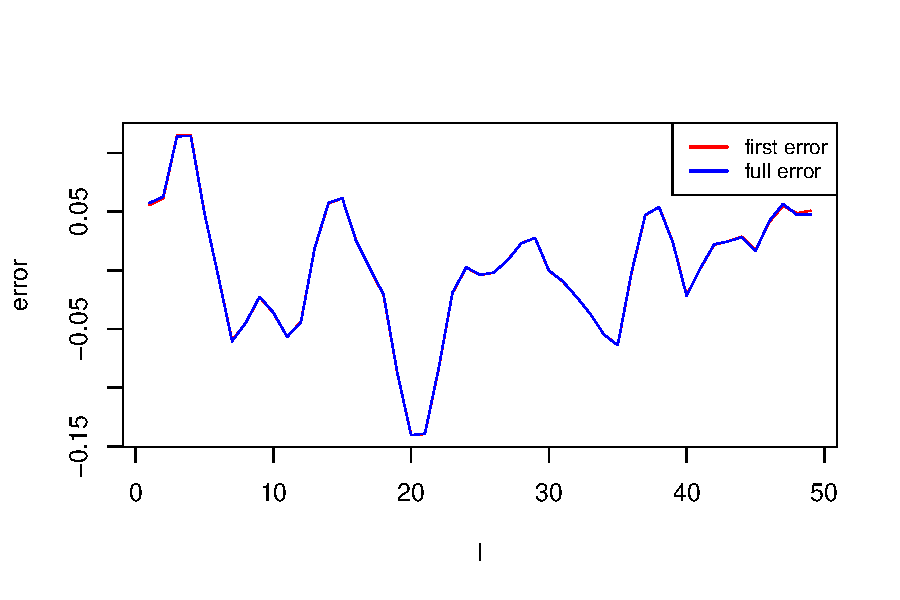
\includegraphics[width=0.6\linewidth]{img/first_vs_full_re.pdf}
		\caption{Вещественные части первого порядка и полной ошибок.}
		\label{fig:harm_noise}
	\end{center}
\end{figure}

Из графика видно, что ошибки практически совпадают даже при маленьком $L$. Аналогичные численные эксперименты подтверждают, что для комплексной экспоненты также есть такое совпадение.

Для случая возмущения в виде выброса был рассмотрен пример с сигналом $s_l = 1 + \iu 1$, с возмущением в виде выброса $a_1 + \iu a_2 = 10 + \iu 10$ на позиции $k = L - 1$. Результаты представлены в таблице~\ref{tab:const_outl}.

\begin{table}[H]
	\begin{center}
		\caption{Максимальное различие первого порядка и полной ошибок.}
		\label{tab:const_outl}
		\begin{tabular}{|c|c|c|c|c|}
			\hline
			$N$	& 50 & 100 & 400 & 1600 \\
			\hline
			$L = N / 2$ & 0.1313  & 0.0419  & 0.0033 & 0.0002 \\
			\hline
			$L = 20$ & 0.3074  & 0.1965  & 0.5655 & 0.6720 \\
			\hline
		\end{tabular}
	\end{center}
\end{table}

Аналогичные численные эксперименты показывают, что при расположении выброса в середине ряда результаты качественно совпадают, при $L = N/2$ различие стремится к $0$, при $L = 20$ не стремится к $0$.

Численные результаты показывают, что для случая зашумленных гармоник первый порядок адекватно оценивает полную ошибку восстановления сигнала в каждой точке при любых рассматриваемых параметрах сигналов.

Однако для случая возмущения в виде выброса это верно, только когда $L$ и $K$ пропорциональны $N$.

Все численные результаты были получены при помощи пакета~\cite{Korobeynikov.etal2014}.

%\begin{figure}[!htb]
%    \centering
%    \begin{subfigure}{.45\textwidth}
%        \centering
%        \includegraphics[width=\textwidth]{img/noise}
%        \caption*{Зашумленный синус.}
%    \end{subfigure}
%    \begin{subfigure}{.45\textwidth}
%        \centering
%        \includegraphics[width=\textwidth]{img/outlier}
%        \caption*{Константа с выбросом.}
%    \end{subfigure}
%    \caption{Сравнение первого порядка ошибки и полной ошибкой.}
%    \label{fig:order1}
%\end{figure}

\section{Заключение}
\label{sec:conclusions}

В работе удалось подвести теоретическую базу под имеющиеся ранее численные результаты (\cite{Golyandina.etal2013}) по сравнению CSSA и SSA для двух зашумленных гармоник с одинаковой частотой и сдвигом, не равным $\pi/2$. Для зашумленной комплексной экспоненты был получен более общий, нежели имеющиеся ранее, численный результат.
Результаты показывают, что только в случае сигнала в виде комплексной экспоненты применение CSSA имеет смысл с точки зрения уменьшения ошибки восстановления сигнала.

Для константного ряда с выбросами был получен явный вид первого порядка ошибок оценки сигнала в каждой точке.

Для обоих случаев было численно исследовано соотношение между первым порядком ошибки и полной ошибкой.
В случае случайного возмущения оказалось, что первый порядок ошибки практически совпадает с полной ошибкой. Однако в случае неслучайного возмущения выбросом это не так и требуются дополнительные условия на пропорциональность длины окна $L$ длине ряда $N$.

\renewcommand\refname{Литература}


\begin{thebibliography}{10}

\bibitem{Golyandina.etal2013}
N.~Golyandina, A.~Korobeynikov, A.~Shlemov, and K.~Usevich.
\newblock Multivariate and {2D} extensions of singular spectrum analysis with
  the {R}ssa package.
\newblock {\em Journal of Statistical Software}, 67(2):1--78, 2015.

\bibitem{Golyandina.etal2001}
N.~Golyandina, V.~Nekrutkin, and A.~Zhigljavsky.
\newblock {\em Analysis of Time Series Structure: {SSA} and Related
  Techniques}.
\newblock Chapman\&Hall/CRC, 2001.

\bibitem{Golyandina.Stepanov2005}
Д.~Степанов, Н.~Голяндина.
\newblock Варианты метода "Гусеница"{-SSA} для прогноза многомерных временных рядов.
\newblock {\em Труды IV Международной конференции "Идентификация систем и задачи управления" { SICPRO'05}}. Москва, 2005, c. 1831-1848.

\bibitem{Korobeynikov.etal2014}
A.~Korobeynikov, A.~Shlemov, K.~Usevich, and N.~Golyandina.
\newblock {\em {Rssa}: A collection of methods for singular spectrum analysis
  {http://CRAN.R-project.org/package=Rssa}}, 2021.
\newblock {R}~package version~1.04.

\bibitem{Kato}
T.~Kato.
\newblock Perturbation theory for linear operators.
\newblock {\em Springer-Verlag,} 1966.

\bibitem{Nekrutkin}
V.~Nekrutkin.
\newblock Perturbation expansions of signal subspaces for long signals.
\newblock {\em Statistics and Its Interface.}, Vol.3, P. 297-319, 2010.

\bibitem{NekrutkinPerp}
V.~Nekrutkin.
\newblock Perturbations in SSA.
\newblock {\em Manuscript}, 2008.

\bibitem{Konstantinov}
А.~Константинов.
\newblock Некоторые задачи анализа временных рядов (теория методов "Singal Subspace").
\newblock {\em Курсовая работа, науч. рук. В.~Некруткин}, 2018.

\end{thebibliography}

\end{document}
